%%%%%%%%%%%%%%%%%%%%%%%%%%%%%%%%%%%%%%%%%%%%%%%%%%%%%%%%%%%%%%%%%%%%%%%%%%%%%%%%%%%%%%%%µ%%%%%%%%%%%
%%%  The State of Linked Data - An Extensible Framework to Validate and Build Dataset Profiles  %%%%
%%%%%%%%%%%%%%%%%%%%%%%%%%%%%%%%%%%%%%%%%%%%%%%%%%%%%%%%%%%%%%%%%%%%%%%%%%%%%%%%%%%%%%%%%%%%%%%%%%%%

\documentclass[runningheads,a4paper]{llncs}

\usepackage[utf8]{inputenc}
\usepackage{amssymb}
\setcounter{tocdepth}{3}
\usepackage{graphicx}
\usepackage{tabularx}
\usepackage{url}
\usepackage{listings}
\usepackage{subfigure}
\usepackage{algorithmic}
\usepackage{algorithm}
\usepackage{xcolor}
\usepackage{multirow}
\usepackage{changepage}


\graphicspath{ {figures/} }

\addtolength{\parskip}{-0.5mm}

\newcommand{\keywords}[1]{\par\addvspace\baselineskip
\noindent\keywordname\enspace\ignorespaces#1}

% todo macro
\usepackage{color}
\newtheorem{deflda}{Axiom}
\newcommand{\todo}[1]{\noindent\textcolor{red}{{\bf \{TODO}: #1{\bf \}}}}

\colorlet{punct}{red!60!black}
\definecolor{background}{HTML}{FFFFFF}
\definecolor{delim}{RGB}{20,105,176}

% Language Definitions for JSON
\lstdefinelanguage{json}{
		basicstyle=\tiny,
    numbersep=4pt,
    showstringspaces=false,
    breaklines=true,
    frame=lines,
    literate=
      {:}{{{\color{punct}{:}}}}{1}
      {,}{{{\color{punct}{,}}}}{1}
      {[}{{{\color{delim}{[}}}}{1}
      {]}{{{\color{delim}{]}}}}{1},
}

%%%%%%%%%%%%%%%%%%%%%%%%%%%%%%%
%%%  Beginning of document  %%%
%%%%%%%%%%%%%%%%%%%%%%%%%%%%%%%

\begin{document}

% first the title is needed
\title{An Extensible Framework to Validate\\ and Build Dataset Profiles}

\author{Ahmad Assaf\inst{1}\inst{2}, Aline Senart\inst{2} and Rapha\"{e}l Troncy\inst{1} }

\institute{EURECOM, Sophia Antipolis, France. \email{<firstName.lastName@eurecom.fr>}
  \and SAP Labs France. \email{<firstName.lastName@sap.com>}
}

% a short form should be given in case it is too long for the running head
\titlerunning{An Extensible Framework to Validate and Build Dataset Profiles}
%\authorrunning{Assaf, Senart and Troncy}

\maketitle

%%%%%%%%%%%%%%%%%%
%%%  Abstract  %%%
%%%%%%%%%%%%%%%%%%

\begin{abstract}
Linked Open Data (LOD) has emerged as one of the largest collections of interlinked datasets on the web. In order to benefit from this mine of data, one needs to access to descriptive information about each dataset (or metadata). This information can be used to delay data entropy, enhance datasets discovery, exploration and reuse as well as helping data portal administrators in detecting and eliminating spam. However, such metadata information is currently very limited to a few data portals where they are usually provided manually, thus being often incomplete and inconsistent in terms of quality. To address these issues, we propose a scalable automatic approach for extracting, validating, correcting and generating descriptive linked dataset profiles. This approach applies several techniques in order to check the validity of the metadata provided and to generate descriptive and statistical information for a particular dataset or for an entire data portal.

% We target CKAN powered data portals and validate our framework on the Linked Open Data (LOD) cloud. The results demonstrate that the general state of LOD cloud needs more attention as most of the datasets suffer from bad quality metadata lacking some informative metrics needed to facilitate dataset search. The noisiest metadata values were access information such as licensing information, resource descriptions as well as resource reachability problems.

\keywords{Linked Data, Dataset Profile, Metadata, Data Quality}
\end{abstract}

%%%%%%%%%%%%%%%%%%%%%%%%%
%%%  1. Introduction  %%%
%%%%%%%%%%%%%%%%%%%%%%%%%

\section{Introduction}
\label{sec:introduction}
From 12 datasets cataloged in 2007, the Linked Open Data cloud has grown to nearly 1000 datasets containing more than 82 billion triples\footnote{http://datahub.io/dataset?tags=lod}~\cite{BizerHeath2009}. Data is being published by both the public and private sectors and covers a diverse set of domains from life sciences to media or government data. The Linked Open Data cloud is potentially a gold mine for organizations and individuals who are trying to leverage external data sources in order to produce more informed business decisions~\cite{Boyd2011}. This success lies in the cooperation between data publishers and consumers. Consumers are empowered to find, share and combine information in their applications easily. However, the heterogeneous nature of data sources reflects directly on the data quality as these sources often contain inconsistent as well as misinterpreted and incomplete metadata information. Considering the significant variation in size, the languages used and the freshness of the data, one realizes that finding useful datasets without prior knowledge is increasingly complicated. This can be clearly noticed in the LOD Cloud where few datasets such as DBPedia~\cite{Bizer:2009:DCP:1640541.1640848}, Freebase~\cite{Bollacker:2008:FCC:1376616.1376746} and YAGO~\cite{Suchanek:2007:YCS:1242572.1242667} are favored over less popular datasets that may include domain specific knowledge more suitable for the tasks at hand. For example, for the task of building context-aware recommender systems in an academic digital library over LOD cloud, popular datasets like Semantic Web Dog Food\footnote{http://datahub.io/dataset/semantic-web-dog-food}, DBLP\footnote{http://datahub.io/dataset/dblp} or Yovisto\footnote{http://datahub.io/dataset/yovisto} can be favored over lesser known but more specific datasets like VIAF\footnote{http://datahub.io/dataset/viaf} which links authority files of 20 national libraries, list of subject headings for public libraries in Spain\footnote{http://datahub.io/dataset/lista-encabezamientos-materia} or the French dissertation search engine\footnote{http://datahub.io/dataset/thesesfr}.

Dataset discovery can be done through public data portals like DataHub\footnote{http://datahub.io} and Europe's Public Data\footnote{http://publicdata.eu} or private ones like Quandl\footnote{https://quandl.com/} or Engima\footnote{http://enigma.io/}. Private portals harness manually curated data from various sources and expose them to users either freely or through paid plans. The data available is of higher quality but lesser quantity compared to what is available in public portals. Similarly, in some public data portals, administrators manually review datasets information, validate, correct and attach suitable metadata information. This information is mainly in the form of predefined tags such as \textit{media, geography, life sciences} for organization and clustering purposes. However, the diversity of those datasets makes it harder to classify them in a fixed number of predefined tags that can be subjectively assigned without capturing the essence and breadth of the dataset~\cite{6690016}. Furthermore, the increasing number of datasets available makes the metadata review and curation process unsustainable even when outsourced to communities.

\textit{Data profiling} is the process of creating descriptive information and collect statistics about that data. It is a cardinal activity when facing an unfamiliar dataset~\cite{semwebprofiling}. Data profiling reflects the importance of datasets without the need for detailed inspection of the raw data.  It also helps in assessing the importance of the dataset, improving users' ability to search and reuse part of the dataset and in detecting irregularities to improve its quality. Data profiling includes typically several tasks:
\begin{itemize}
  \item \textbf{Metadata profiling}: Provides general information on the dataset (dataset description, release and update dates), legal information (license information, openness), practical information (access points, data dumps), etc.
  \item \textbf{Statistical profiling}: Provides statistical information about data types and patterns in the dataset, i.e., properties distribution, number of entities and RDF triples, etc.
  \item \textbf{Topical profiling}: Provides descriptive knowledge on the dataset content and structure. This can be in form of tags and categories used to facilitate search and reuse.
\end{itemize}

In this work, we address the challenges of automatic validation and generation of descriptive datasets profiles. This paper proposes Roomba, an extensible framework consisting of a processing pipeline that combines techniques for data portals identification, datasets crawling and a set of pluggable modules combining several profiling tasks. The framework validates the provided dataset metadata against an aggregated standard set of information. Metadata fields are automatically corrected when possible, e.g., adding a missing license URL reference. Moreover, a report describing all the issues highlighting those that cannot be automatically fixed is created to be sent by email to the dataset's maintainer. There exist various statistical and topical profiling tools for both relational and Linked Data. The architecture of the framework allows to easily add them as additional profiling tasks. However, in this paper, we focus on the task of dataset metadata profiling. We validate our framework against a manually created set of profiles and manually check its accuracy by examining the results of running it on various CKAN-based data portals.

The remainder of the paper is structured as follows. In Section~\ref{sec:motivation}, we present the motivation behind our framework. In Section~\ref{sec:related-work}, we review relevant related work. In Section~\ref{sec:framework}, we describe our proposed framework's architecture and components that validate and generate dataset profiles. In Section~\ref{sec:experiment}, we evaluate the framework and we finally conclude and outline some future work in Section~\ref{sec:conclusion}.

%%%%%%%%%%%%%%%%%%%%%%%%%
%%%  2. Motivation  %%%
%%%%%%%%%%%%%%%%%%%%%%%%%
\section{Motivation}
\label{sec:motivation}

Metadata provisioning is one of the Linked Data publishing best practices mentioned in \cite{Bizer:2011:EWG:2075914.2075915}. Datasets should contain the metadata needed to effectively understand and use them. This information includes the dataset's license, provenance, context, structure and accessibility. The ability to automatically check this metadata helps in:

\begin{itemize}
  \item \textbf{Delaying data entropy}: \textit{Information entropy} refers to the degradation or loss limiting the information content in raw or metadata. As a consequence of information entropy, data complexity and dynamicity, the life span of data can be very short. Even when the raw data is properly maintained, it is often rendered useless when the attached metadata is missing, incomplete or unavailable. Comprehensive high quality metadata can counteract these factors and increase dataset longevity~\cite{GTOS}.
  \item \textbf{Enhancing data discovery, exploration and reuse}: Users who are unfamiliar with a dataset require detailed metadata to interpret and analyze accurately unfamiliar datasets. A study conducted by the European Union commission~\cite{Graham:11:}, found that both business and users are facing difficulties in discovering, exploring and reusing public data. due to missing or inconsistent metadata information.
  \item \textbf{Enhancing spam detection}: Portals hosting public open data like Datahub allow anyone to freely publish datasets. Even with security measures like captchas and anti-spam devices, detecting spam is increasingly difficult. In addition to that, the increasing number of datasets hinders the scalability of this process, affecting the correct and efficient spotting of datasets spam.
\end{itemize}

%%%%%%%%%%%%%%%%%%%%%%%%%
%%%  3. Related Work  %%%
%%%%%%%%%%%%%%%%%%%%%%%%%

\section{Related Work}
\label{sec:related-work}

Data Catalog Vocabulary (DCAT) \cite{Erickson:14:DCV} and the Vocabulary of Interlinked Datasets (VoID) \cite{Cyganiak:11:DLD} are concerned with metadata about RDF datasets. There exist several tools aiming at exposing dataset metadata using these vocabularies. In \cite{BoHm:2011:CVD:2030805.2031001} authors generate VoID descriptions limited to a subset of properties that can be automatically deduced from resources within the dataset. However, it still provides data consumers with interesting insights. Quality Assessment of Data Sources (Flemming's Data Quality Assessment Tool)\footnote{http://linkeddata.informatik.hu-berlin.de/LDSrcAss/datenquelle.php} provides basic metadata assessment as it calculates data quality scores based on manual user input. The user assigns weights to the predefined quality metrics and answer a series of questions regarding the dataset. These include, for example, the use of obsolete classes and properties by defining the number of described entities that are assigned disjoint classes, the usage of stable URIs and whether the publisher provides a mailing list for the dataset. The ODI certificate\footnote {https://certificates.theodi.org/} on the other hand provides a description of the published data quality in plain English. It aspires to act as a mark of approval that helps publishers understand how to publish good open data and users how to use it. It gives publishers the ability to provide assurance and support on their data while encouraging further improvements through an ascending scale. ODI comes as an online and free questionnaire for data publishers focusing on certain characteristics about their data. Although these approaches try to perform metadata profiling, they are either incomplete or manual. In our framework, we propose a more automatized and complete approach.

\textbf{Metadata profiling}: The Project Open Data Dashboard\footnote{http://labs.data.gov/dashboard/} tracks and measures how US government websites implement the Open Data principles to understand the progress and current status of their public data listings. A validator analyzes machine readable files e.g., JSON files for automated metrics like the resolved URLs, HTTP status and content-type. However, deep schema information about the metadata is missing like description, license information or tags. Similarly on the LOD cloud, the Data Hub LOD Validator\footnote{http://validator.lod-cloud.net/} gives an overview of Linked Data sources cataloged on the Data Hub. It offers a step-by-step validator guidance to check a dataset completeness level for inclusion in the LOD cloud. The results are divided into four different compliance levels from basic to reviewed and included in the LOD cloud. Although it is an excellent tool to monitor LOD compliance, it still lacks the ability to give detailed insights about the completeness of the metadata and overview on the state of the whole LOD cloud group and is very specific to the LOD cloud group rules and regulations.

\textbf{Statistical profiling}: Calculating statistical information on datasets is vital to applications dealing with query optimization and answering, data cleansing, schema induction and data mining \cite{profilingWebOfData} \cite{datafinland2} \cite{6690016}. Semantic sitemaps \cite{Cyganiak:2008:SSE:1789394.1789457} and RDFStats \cite{Langegger:2009:RER:1674635.1674691} where one of the first to deal with RDF data statistics and summaries. ExpLOD \cite{Khatchadourian:2010:ESE:2155278.2155300} creates statistics on the interlinking between datasets based on \texttt{owl:sameAs} links. In \cite{semwebprofiling} the author introduces a tool that induces the actual schema of the data and gather corresponding statistics accordingly. LODStats  \cite{Auer:2012:LEF:2413941.2413982} is a stream-based approach that calculates more general dataset statistics. ProLOD++ \cite{6816740} is a Web-based tool that allows LOD analysis via automatically computed hierarchical clustering \cite{5452762}. Aether \cite{makela-aether-2014} generates VoID statistical descriptions of RDF datasets. It also provides a Web interface to view and compare VoID descriptions. LODOP \cite{forchhammer_profiles_2014} is a MapReduce framework to compute, optimize and benchmark dataset profiles. The main target for this framework is to optimize the runtime costs for Linked Data profiling. In \cite{DyLDO} authors calculate certain statistical information for the purpose of observing the dynamic changes in datasets.

\textbf{Topical Profiling}: Topical and categorical information facilitates dataset search and reuse. Topical profiling focuses on content-wise analysis at the instances and ontological levels. GERBIL \cite{gerbil} is a general entity annotation framework that provides machine processable output allowing efficient querying. In addition, there exist several entity annotation tools and frameworks \cite{Cornolti:2013:FBE:2488388.2488411} but none of those systems are designed specifically for dataset annotation. In \cite{datafinalnd}, authors created a semantic portal to manually annotate and publish metadata about both LOD and non-RDF datasets. In \cite{6690016}, authors automatically assigned Freebase domains to extracted instance labels of some of the LOD Cloud datasets. The goal was to provide automatic domain identification, thus enabling improving datasets clustering and categorization. In \cite{Bohm:2012:LTG:2396761.2398718}, authors extracted dataset topics by exploiting the graph structure and ontological information, thus removing the dependency on textual labels. In  \cite{scalableApproach} authors generate VoID and VoL descriptions via a processing pipeline that extracts dataset topic models ranked on graphical models of selected DBpedia categories.

\textbf{Dataset Search}:Dataset search can be done without relying on attached metadata (tags and categories). For example, there exist several approaches to create LOD indexes. In \cite{Alexander:LDOW09}, authors used VoID descriptions to optimize query processing by determining relevant query-able datasets. In \cite{Harth:2010:DSO:1772690.1772733}, authors created an approximate index structure (QTree) and an algorithm for answering conjunctive queries over Linked Data. SchemEX \cite{Konrath:2012:SEC:2399444.2399563} is a stream-based approach leveraging type and property information of RDF instances to create schema-level indexes.\\
Semantic search engines like Sindice \cite{Delbru2010a}, Swoogle \cite{Ding2004} and Watson \cite{d'Aquin:2011:WMS:2019470.2019476} help in entities lookup but are not designed specifically for dataset search. In \cite{whatShouldILinkTo}, authors utilized the sig.ma index \cite{sig.ma} to identify appropriate data sources for interlinking. Dataset search and discovery is currently done via data portals that rely on attached metadata to provide dataset search features as they run a Solr index on the metadata schemas. Having missing or inconsistent information will affect the search results quality.

Although the above mentioned tools are able to provide various types of information about a dataset, there exists no approach that aggregates this information and is extensible to combine additional profiling tasks. To the best of our knowledge, this is the first effort towards extensible automatic validation and generation of descriptive dataset profiles.

%%%%%%%%%%%%%%%%%%%%%%%%%%%%%%%%%%%
%%%  4. Profiling data portals  %%%
%%%%%%%%%%%%%%%%%%%%%%%%%%%%%%%%%%%

\section{Profiling Data Portals}
\label{sec:framework}

In this section, we provide an overview of Roomba's architecture and the processing steps for validating and generating dataset profiles. Figure \ref{fig:1} shows the main steps which are the following: (i) data portal identification; (ii) metadata extraction; (iii) instance and resource extraction; (iv) profile validation (v) profile and report generation.

Roomba is built as a Command Line Interface (CLI) application using Node.js. Instructions on installing and running the framework are available on its public Github repository\footnote{https://github.com/ahmadassaf/opendata-checker}. The various steps are explained in detail below.

\begin{figure}[!ht]
  \centering
    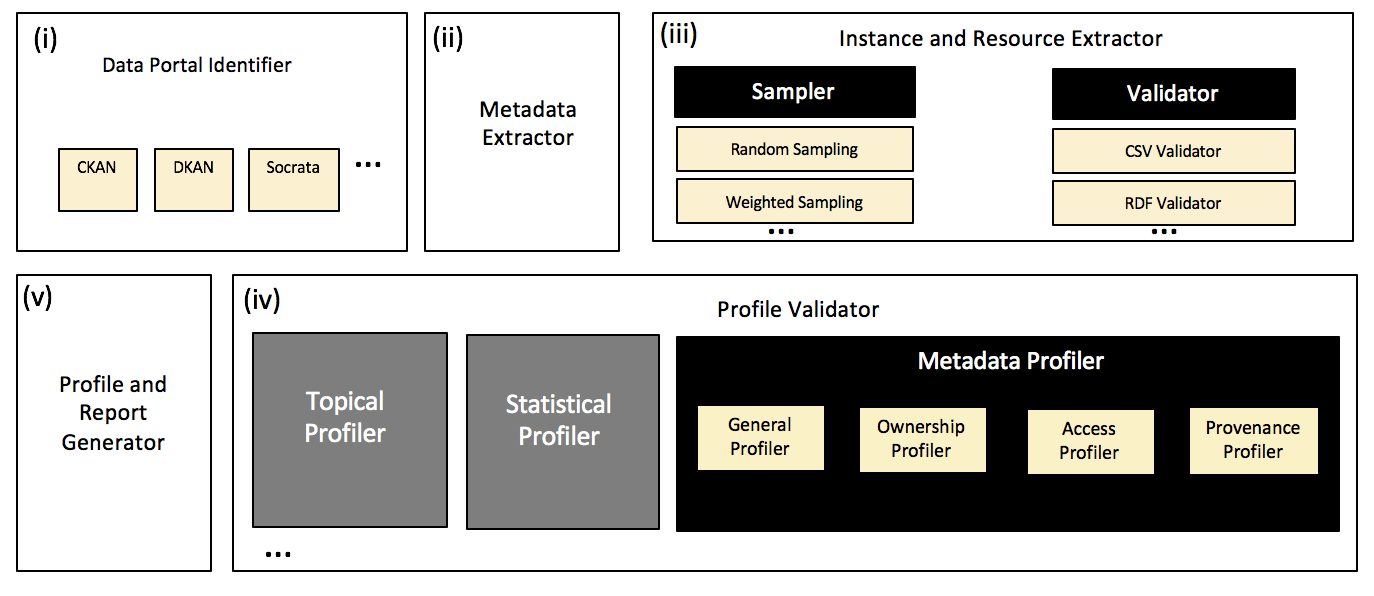
\includegraphics[scale=0.4]{figure-1_architecture.png}
  \caption{Processing pipeline for validating and generating dataset profiles}
  \label{fig:1}
\end{figure}

\subsection{Data Portal Identification}

Data portals can be considered as data access points providing tools to facilitate data publishing, sharing, searching and visualization. CKAN\footnote{http://ckan.org} is the world's leading open-source data portal platform powering websites like DataHub, Europe's Public Data and the U.S Government's open data. Modeled on CKAN, DKAN\footnote{http://drupal.org/project/dkan} is a standalone Drupal distribution that is used in various public data portals as well. Socrata\footnote{http://www.socrata.com} helps public sector organizations improve data-driven decision making by providing a set of solutions including an open data portal. In addition to these tradition data portals, there is a set of tools that allow exposing data directly as RESTful APIs like Datatank\footnote{http://thedatatank.com} and Database-to-API\footnote{https://github.com/project-open-data/db-to-api}.

Roomba should be extensible to any data portal. Since every portal has its own API and data model, identifying the software powering data portals is a vital first step. We rely on several Web scraping techniques in the identification process which includes a combination of the following:

\begin{itemize}
  \item \textbf{URL inspection}: Various CKAN based portals are hosted on subdomains of the \texttt{http://ckan.net}. For example, CKAN Brazil (\texttt{http://br.ckan.net}). Checking the existence of certain URL patterns can detect such cases.
  \item \textbf{Meta tags inspection}: The \texttt{<meta>} tag provides metadata about the HTML document. They are used to specify page description, keywords, author, etc. Inspecting the \texttt{content} attribute can indicate the type of the data portal. We use CSS selectors to check the existence of these meta tags. An example of a query selector is \texttt{meta[content*="ckan]} (all meta tags with the attribute content containing the string $CKAN$). This selector can identify CKAN portals whereas the \texttt{meta[content*="Drupal"]} can identify DKAN portals.
  \item \textbf{Document Object Model (DOM) inspection}: Similar to the meta tags inspection, we check the existence of certain DOM elements or properties. For example, CKAN powered portals will have DOM elements with class names like \texttt{ckan-icon} or \texttt{ckan-footer-logo}. A CSS selector like \texttt{.ckan-icon} will be able to check if a DOM element with the class name \texttt{ckan-icon} exists.
  The list of elements and properties to inspect is stored in a separate configurable object for each portal. This allows the addition and removal of elements as deemed necessary.
\end{itemize}

The identification process for each portal can be easily customized by overriding the default function. Moreover, adding or removing steps from the identification process can be easily configured.

After those preliminary checks, we query one of the portal's API endpoints. For example, DataHub is identified as CKAN, so we will query the API endpoint on \texttt{http://datahub.io/api/action/package\_list}. A successful request will list the names of the site's datasets, whereas a failing request will signal a possible failure of the identification process.

\subsection{Metadata Extraction}

Data portals expose a set of information about each dataset as metadata. The model used varies across portals. However, a standard model should contain information about the dataset's title, description, maintainer email, update and creation date, etc. We divided the metadata information into the following types:

\textbf{General information}: General information about the dataset. e.g., title, description, ID, etc. This general information is manually filled by the dataset owner. In addition to that, tags and group information is required for classification and enhancing dataset discoverability. This information can be entered manually or inferred modules plugged into the topical profiler.

\textbf{Access information}: Information about accessing and using the dataset. This includes the dataset URL, license information i.e., license title and URL and information about the dataset's resources. Each resource has as well a set of attached metadata e.g., resource name, URL, format, size, etc.

\textbf{Ownership information}: Information about the ownership of the dataset. e.g., organization details, maintainer details, author, etc. The existence of this information is important to identify the authority on which the generated report and the newly corrected profile will be sent to.

\textbf{Provenance information}: Temporal and historical information on the dataset and its resources. For example, creation and update dates, version information, version, etc. Most of this information can be automatically filled and tracked.

Building a standard metadata model is not the scope of this paper, and since we focus on CKAN-based portals, we validate the extracted metadata against the CKAN standard model\footnote{http://demo.ckan.org/api/3/action/package\_show?id=adur\_district\_spending}.

After identifying the underlying portal software, we perform iterative queries to the API in order to fetch datasets metadata and persist them in a file-based cache system.
Depending on the portal software we can issue specific extraction jobs. For example, in CKAN based portals, we are able to crawl and extract the metadata of a specific dataset, all the datasets in a specific group e.g., LOD Cloud or all the datasets in the portal.

\subsection{Instance and Resource Extraction}

From the extracted metadata we are able to identify all the resources associated with that dataset. They can have various types like a SPARQL endpoint, API, file, visualization, etc. However, before extracting the resource instance(s) we perform the following steps:

\begin{itemize}
  \item \textbf{Resource metadata validation and enrichment}: Check the resource attached metadata values. Similar to the dataset metadata, each resource should include information about its mimetype, name, description, format, valid de-referenceable URL, size, type and provenance. The validation process issue an HTTP request to the resource and automatically fills up various missing information when possible, like the mimetype and size by extracting them from the HTTP response header. However, missing fields like name and description that needs manual input are marked as missing and will appear in the generated summary report.
  \item \textbf{Format validation}: Validate specific resource formats against a linter or a validator. For example, node-csv\footnote{https://github.com/wdavidw/node-csv} for CSV files and n3\footnote{https://github.com/RubenVerborgh/N3.js} to validate N3 and Turtle RDF serializations.
\end{itemize}

Considering that certain datasets contain large amounts of resources and the limited computation power of some machines on which the framework might run on, a sampler module can be introduced to execute various sample-based strategies detailed as they were found to generate accurate results even with comparably small sample size of 10\%. These strategies introduced in \cite{scalableApproach} are:

\begin{itemize}
  \item \textbf{Random Sampling}: Randomly selects resources instances.
  \item \textbf{Weighted Sampling}: Weighs each resources as the ratio of the number of datatype properties used to define a resource over the maximum number of datatype properties over all the datasets resources.
  \item \textbf{Resource Centrality Sampling}: Weighs each resource as the ration of the number of resource types used to describe a particular resource divided by the total number of resource types in the dataset. This is specific and important to RDF datasets where important concepts tend to be more structured and linked to other concepts.
\end{itemize}

However, the sampler is not restricted only to these strategies. Strategies like those introduced in \cite{Leskovec:2006:SLG:1150402.1150479} can be configured and plugged in the processing pipeline.

\subsection{Profile Validation}

A dataset profile should include descriptive information about the data examined. In our framework, we have identified three main categories of profiling information. However, the extensibility of our framework allows for additional profiling techniques to be plugged in easily i.e., a quality profiling module reflecting the dataset quality. In this paper, we focus on the task of metadata profiling.

Metadata validation process identifies missing information and the ability to automatically correct them. Each set of metadata (general, access, ownership and provenance) is validated and corrected automatically when possible. Each profiler task has a set of metadata fields to check against. The validation process check if each field is defined and if the value assigned is valid.

There exist a bunch of special validation steps for various fields. For example, the email addresses and urls should be validated to ensure that the value entered is syntactically correct. In addition to that, for urls, we issue an HTTP \texttt{HEAD} request in order to check if that URL is reachable. We also use the information contained in a valid \texttt{content-header} response to extract, compare and correct some resources metadata values like \texttt{mimetype} and \texttt{size}.

Despite the legal issues surrounding Linked Data licenses \cite{nomoneyLOD}, it is still considered a gold mine for organizations who are trying to leverage external data sources in order to produce more informed business decisions \cite{Boyd2011}. In \cite{mckinseyreport} the authors see the potential economic effect unfolding in education, transportation, consumer products, electricity, oil and gas, health care and consumer finance. They estimate the potential annual value enabled by Open Data in these domains to be 3 trillion US Dollars across seven domains. As a result, validating license related information is vital. However, from our experiments, we found out that datasets' license information is noisy. The license names if found are not standardized. For example, Creative Commons CCZero can be also CC0 or CCZero. Moreover,the license URI if found and if de-referenceable can point to different reference knowledge bases e.g., \texttt{http://opendefinition.org}. To overcome this issue, we have manually created a mapping file standardizing the set of possible license names and the reference knowledge base\footnote{https://github.com/ahmadassaf/opendata-checker/blob/master/util/licenseMappings.json}. In addition, we have also used the open source and knowledge license information\footnote{https://github.com/okfn/licenses} to normalize the license information and add extra metadata like the domain, maintainer and open data conformance.

\lstset{frame=single, caption={License mapping file sample}, label=json, captionpos=b}
\begin{lstlisting}[language=json]
{
	"license_id" : ["ODC-PDDL-1.0"],
	"disambiguations" : ["Open Data Commons Public Domain Dedication and License (PDDL)"]
},
{
	"license_id" : ["CC-BY-SA-4.0", "CC-BY-SA-3.0"],
	"disambiguations" : ["cc-by-sa", "CC BY-SA","Creative Commons Attribution Share-Alike"]
}
\end{lstlisting}

% \textbf{Statistical profiling}\\

% There exist a set of tools designed specifically to provide statistical information about a dataset (see section 2). Providing comprehensive statistical information about a dataset isn't in the scope of this paper. However, to show the extensibility of our framework we provide a simple RDF statistical profiler module that can be easily extended and configured. The information provided for each class is the number: triples, distinct objects, distinct literals, distinct IRI reference objects, distinct blank nodes objects, distinct subjects, distinct IRI reference subjects and distinct blank nodes subjects.\\

% \textbf{Topical profiling}\\

% Similar to the statistical profiler, a detailed survey of the existing tools can be found in the related work section. However, we implement a very basic topical profiler by applying Named Entity Disambiguation (NED) on the textual description and title of a dataset using DBpedia Spotlight \cite{Mendes:2011:DSS:2063518.2063519}.

\subsection{Profile and Report Generation}

The validation process highlights the missing information and presents them in a human readable report. The report can be automatically sent to the dataset maintainer email if exists in the metadata.

In addition to the generated report, the enhanced profiles are represented in JSON using the CKAN data model and are publicly available\footnote{https://github.com/ahmadassaf/opendata-checker/tree/master/results}.

Data portal administrators need an overall knowledge of the portal datasets and their properties. Our framework has the ability to generate numerous reports of all the datasets by passing formated queries. There are two main sets of aggregation tasks that can be run:
\begin{itemize}
  \item \textbf{Aggregating meta-field values}: Passing a string that corresponds to a valid field in the metadata. The field can be flat like \texttt{license\_title} (aggregates all the license titles used in the portal or in a specific group) or nested like \texttt{resource>resource\_type} (aggregates all the resources types for all the datasets). Such reports are important to have an overview of the possible values used for each metadata field.
  \item \textbf{Aggregating key:object meta-field values}: Passing two meta-field values separated by a colon \texttt{:} e.g., \texttt{resources>resource\_type:resources>name}. These reports are important as you can aggregate the information needed when also having the set of values associated to it printed.
\end{itemize}

For example, the meta-field value query \texttt{resource>resource\_type} run against the LODCloud group will result in an array containing $[file,api,documentation ...]$ values. These are all the resource types used to describe all the datasets of the group. However, to be able to know also what are the datasets containing resources corresponding to each type, we issue a key:object meta-field query \texttt{resource>resource\_type:name}. The result will be a JSON object having the \texttt{resource\_type} as the key and an array of corresponding datasets titles that has a resource of that type.

\lstset{basicstyle=\scriptsize, backgroundcolor=\color{white}, breaklines=true, frame=single, caption={Excerpt of the DBpedia validation report}, label=report, captionpos=b}
\begin{lstlisting}
 =======================================================================
                          Metadata Report
 =======================================================================
  group information is missing. Check organization information as they can be mixed sometimes
  organization_image_url field exists but there is no value defined
 =======================================================================
                          Tag Statistics
 =======================================================================
  There is a total of: 21 [undefined] vocabulary_id fields  100.00%
 =======================================================================
                          License Report
 =======================================================================
  License information has been normalized !
 =======================================================================
                        Resource Statistics
 =======================================================================
  There is a total of: 10 [missing] url-type fields  100.00%
  There is a total of: 9 [missing] created fields  90.00%
  There is a total of: 10 [undefined] cache_last_updated fields  100.00%
  There is a total of: 10 [undefined] size fields  100.00%
  There is a total of: 10 [undefined] hash fields  100.00%
  There is a total of: 10 [undefined] mimetype_inner fields  100.00%
  There is a total of: 7 [undefined] mimetype fields  70.00%
  There is a total of: 10 [undefined] cache_url fields  100.00%
  There is a total of: 6 [undefined] name fields  60.00%
  There is a total of: 9 [undefined] webstore_url fields  90.00%
  There is a total of: 9 [undefined] last_modified fields  90.00%
  There is one [undefined] format field  10.00%
 =======================================================================
                   Resource Connectivity Issues
 =======================================================================
  There are 2 connectivity issues with the following URLs:
    - http://dbpedia.org/void/Dataset
 =======================================================================
                     Un-Reachable URLs Types
 =======================================================================
  There are: 1 unreachable URLs of type [file]
\end{lstlisting}

%%%%%%%%%%%%%%%%%%%%%%%%%%%%%%%%%%%%%%%
%%%  5. Experiments and Evaluation  %%%
%%%%%%%%%%%%%%%%%%%%%%%%%%%%%%%%%%%%%%%

\section{Experiments and Evaluation}
\label{sec:experiment}

In this section, we provide the experiments and evaluation of the proposed framework. All the experiments are reproducible by our tool and their results are available in its Github repository.

A CKAN dataset metadata describes four main sections in addition to the core dataset's properties. These sections are:

\begin{itemize}
  \item \textbf{Resources}: The distributable parts containing the actual raw data. They can come in various formats (JSON, XML, RDF, etc.) and can be downloaded or accessed directly (REST API, SPARQL endpoint).
  \item \textbf{Tags}: Provide descriptive knowledge on the dataset content and structure. They are used mainly to facilitate search and reuse.
  \item \textbf{Groups}: A dataset can belong to one or more group that share common semantics. A group can be seen as a cluster or a curation of datasets based on shared categories or themes.
  \item \textbf{Organizations}: A dataset can belong to one or more organization controlled by a set of users. Organizations are different from groups as they are not constructed by shared semantics or properties, but solely on their association to a specific administration party.
\end{itemize}

Each of these sections contains a set of metadata corresponding to one or more type (general, access, ownership and provenance). For example, a dataset resource will have general information such as the resource name, access information such as the resource url and provenance information such as creation date. The framework generates a report aggregating all the problems in all these sections, fixing field values when possible. Errors can be the result of missing metadata fields, undefined field values or field value errors e.g., unreachable URL or incorrect email addresses.

\subsection{Experimental Setup}

We ran our tool on two CAKN-based data portals. The first is the Datahub targeting specifically the LOD cloud group. The current state of the LOD cloud report~\cite{DBLP:conf/semweb/SchmachtenbergBP14} indicates that the LOD cloud contains 1014 datasets. They were harvested via an LDSpider crawler~\cite{conf/semweb/IseleUBH10} seeded with 560 thousands URIs. Roomba on the other hand, fetches datasets hosted in data portals where datasets have attached relevant metadata. As a result, we relied on the information provided by the Datahub CKAN API. Examining the tags available, we found two candidate groups. The first tagged with "lodcloud" returned 259 datasets, while the second tagged with "lod" returned only 75 datasets. After manually examining the two lists, we found out the datasets grouped with the tag "lodcloud" are the correct ones. To qualify other CKAN-based portals for the experiments, we used \texttt{dataportals.org}, which contains a comprehensive list of Open Data portals from around the world. In the end, we chose the Amsterdam data portal \footnote{http://data.amsterdamopendata.nl/}. The portal was commissioned in 2012 by the Amsterdam Economic Board Open Data Exchange (ODE), and covers a wide range of information domains (energy, economy, education, urban development, etc.) about Amsterdam metropolitan region.

We ran the instance and resource extractors in order to cache the metadata files for these datasets locally and ran the validation process. The experiments were executed on a 2.6 Ghz Intel Core i7 processor with 16GB of DDR3 memory machine. The approximate execution time alongside  the summary of the datasets' properties are presented in table \ref{tab:dataportals}.

\begin{table}[ht]
\centering
\begin{tabular}{|l|c|c|c|c|}
\hline
Data Portal         & \multicolumn{1}{l|}{No. Datasets} & \multicolumn{1}{l|}{No. Groups} & \multicolumn{1}{l|}{No. Resources} & \multicolumn{1}{l|}{Processing Time} \\ \hline
LOD Cloud           & 259                               & N/A                            & 1068                               & ~140 mins                            \\ \hline
Amsterdam Open Data & 172                               & 18                             & 480                                & ~35 mins                             \\ \hline
\end{tabular}
\caption{Summary of the experiments details}
\label{tab:dataportals}
\end{table}

In our evaluation, we focused on two aspects: i)\textit{profiling correctness} which assesses the validity of the errors generated in report manually, and ii)\textit{profiling completeness} which assesses if the profilers cover all the errors in the datasets metadata.

\subsection{Profiling Correctness}

To measure profile correctness, we need to make sure that the issues reported by Roomba are valid on the dataset, group and portal levels.

On the dataset level, we choose three datasets from both the LOD Cloud and the Amsterdam data portal. The datasets details are shown in table \ref{tab:datasesExperiment}.

\begin{table}[ht]
\centering
\footnotesize\setlength{\tabcolsep}{1.5pt}
\begin{tabular}{|l|c|c|c|c|}
\hline
\textbf{Dataset Name}          & \multicolumn{1}{l|}{\textbf{Data Portal}} & \multicolumn{1}{l|}{\textbf{Group ID}} & \multicolumn{1}{l|}{\textbf{Resources}} & \multicolumn{1}{l|}{\textbf{Tags}} \\ \hline
dbpedia                        & Datahub                                   & lodcloud                               & 10                                      & 21                                 \\ \hline
event-media                    & Datahub                                   & lodcloud                               & 9                                       & 15                                 \\ \hline
bbc-music                      & Datahub                                   & lodcloud                               & 2                                       & 14                                 \\ \hline
bevolking\_cijfers\_amsterdam  & Amsterdam                                 & bevolking                              & 6                                       & 12                                 \\ \hline
bevolking-prognoses-amsterdam  & Amsterdam                                 & bevolking                              & 1                                       & 3                                  \\ \hline
religieuze\_samenkomstlocaties & Amsterdam                                 & bevolking                              & 1                                       & 8                                  \\ \hline
\end{tabular}
\caption{Datasets chosen for the correctness evaluation}
\label{tab:datasesExperiment}
\end{table}

To measure the profiling correctness on the groups level, we selected four groups from the Amsterdam data portal containing a total of 25 datasets. The choice was made to cover groups in various domains that contain a moderate number of datasets that can be checked manually (between 3-9 datasets). Table \ref{tab:groups} summarizes the groups chosen for the evaluation.

\begin{table}[ht]
\centering
\begin{tabular}{|l|c|c|c|c|}
\hline
\textbf{Group Name}      & \textbf{Domain}        & \multicolumn{1}{l|}{\textbf{Datasets}} & \multicolumn{1}{l|}{\textbf{Resources}} & \multicolumn{1}{l|}{\textbf{Tags}} \\ \hline
bestuur-en-organisatie   & Management             & 9                                      & 45                                      & 101                                \\ \hline
bevolking                & Population             & 3                                      & 8                                       & 23                                 \\ \hline
geografie                & Geography              & 8                                      & 16                                      & 56                                 \\ \hline
openbare-orde-veiligheid & Public Order \& Safety & 5                                      & 19                                      & 34                                 \\ \hline
\end{tabular}
\caption{Groups chosen for the correctness evaluation}
\label{tab:groups}
\end{table}

After running Roomba and examining the results on the selected datasets and groups, we found out that our framework provides 100\% correct results on the individual dataset level and on the aggregation level over groups. Since our portal level aggregation is extended from the group aggregation we can infer that the portal level aggregation also produces complete correct profiles. However, the lack of a standard way to create and manage collections of datasets was the source of some errors when comparing the results from these two portals. For example, in Datahub, we noticed that all the datasets \texttt{groups} information were missing, while in the Amsterdam Open Data portal, all the \texttt{organisation} information was missing. Although the error detection is correct, the overlap in the usage of group and organization can give a false indication about the metadata quality.

\subsection{Profiling Completeness}

We analyzed the completeness of our framework by manually constructing a set of profiles that act as a golden standard. These profiles cover the range of uncommon problems that can occur in a certain dataset\footnote{https://github.com/ahmadassaf/opendata-checker/tree/master/test}. These errors are:

\begin{itemize}
\item Incorrect \texttt{mimetype} or \texttt{size} for resources
\item Invalid number of tags or resources defined
\item Check if the license information can be normalized via the \texttt{license\_id} or the \texttt{license\_title} as well as the normalization result.
\item Syntacticly invalid \texttt{author\_email} or \texttt{maintainer\_email}.
\end{itemize}


After running our framework at each of these profiles, we measured the completeness and correcteness of the results. We found out that our framework covers indeed all the metadata problems that can be found in a CKAN standard model correctly.

%%%%%%%%%%%%%%%%%%%%%%%%%%%%%%%%%%%%%%%
%%%  6. Conclusion and Future Work  %%%
%%%%%%%%%%%%%%%%%%%%%%%%%%%%%%%%%%%%%%%
\section{Conclusion and Future Work}
\label{sec:conclusion}

In this paper, we proposed a scalable automatic approach for extracting, validating, correcting and generating descriptive linked dataset profiles. This approach applies several techniques in order to check the validity of the metadata provided and to generate descriptive and statistical information for a particular dataset or for an entire data portal. Based on our experiments running the tool on the LOD cloud, we discovered that the general state of the datasets needs attention as most of them lack informative access information and their resources suffer low availability. These two metrics are of high importance for enterprises looking to integrate and use external linked data.

It has been noticed that the issues surrounding metadata quality affect directly dataset search as data portals rely on such information to power their search index. We noted the need for tools that are able to identify various issues in this metadata and correct them automatically. We evaluated our framework manually against two prominent data portals and proved that we can automatically scale the validation of datasets metadata profiles completely and correctly.

As part of our future work, we plan to introduce workflows that will be able to correct the rest of the metadata either automatically or through intuitive manually-driven interfaces. We also plan to integrate statistical and topical profilers to be able to generate full comprehensive profiles. We also intend to suggest a ranked standard metadata model that will help generate more accurate and scored metadata quality profiles. We also plan to run this tool on various CKAN based data portals, schedule periodic reports to monitor the evolvement of datasets metadata. Finally, at some stage, we plan to extend this tool for other data portal types like DKAN and Socrata.

%%%%%%%%%%%%%%%%%%%%%%%%%
%%%  Acknowledgments  %%%
%%%%%%%%%%%%%%%%%%%%%%%%%

\section*{Acknowledgments}
This research has been partially funded by the European Union's 7th Framework Programme via the project Apps4EU (GA No. 325090).
\vspace{0.5cm}

\bibliographystyle{abbrv}
\nocite{*}
\bibliography{SOLD}
\end{document}
